\documentclass{beamer}
\mode<presentation>
\usepackage{amsmath,amssymb,mathtools}
\usepackage{textcomp}
\usepackage{gensymb}
\usepackage{adjustbox}
\usepackage{subcaption}
\usepackage{enumitem}
\usepackage{multicol}
\usepackage{listings}
\usepackage{url}
\usepackage{graphicx} % <-- needed for images
\def\UrlBreaks{\do\/\do-}

\usetheme{Boadilla}
\usecolortheme{lily}
\setbeamertemplate{footline}{
  \leavevmode%
  \hbox{%
  \begin{beamercolorbox}[wd=\paperwidth,ht=2ex,dp=1ex,right]{author in head/foot}%
    \insertframenumber{} / \inserttotalframenumber\hspace*{2ex}
  \end{beamercolorbox}}%
  \vskip0pt%
}
\setbeamertemplate{navigation symbols}{}

\lstset{
  frame=single,
  breaklines=true,
  columns=fullflexible,
  basicstyle=\ttfamily\tiny
}

\numberwithin{equation}{section}

% ---- your macros ----
\providecommand{\myvec}[1]{\ensuremath{\begin{pmatrix}#1\end{pmatrix}}}
\newenvironment{amatrix}[1]{%
  \left(\begin{array}{@{}*{#1}{c}|c@{}}
}{%
  \end{array}\right)
}
\newcommand{\myaugvec}[2]{\ensuremath{\begin{amatrix}{#1}#2\end{amatrix}}}
\let\vec\mathbf
% ---------------------

\title{Matgeo Presentation - System of 3 Equations}
\author{EE25BTECH11048 - Revanth Siva Kumar}

\begin{document}

% -------------------
\begin{frame}
  \titlepage
\end{frame}

% -------------------
\begin{frame}{Problem Statement}
Solve the system of equations
\[
\begin{aligned}
5x - y + 4z &= 5\\
2x + 3y + 5z &= 2\\
5x - 2y + 6z &= -1
\end{aligned}
\]
\end{frame}

% -------------------
\begin{frame}{Data}
\begin{table}[h!]
  \centering
  \begin{tabular}{|c|c|}
\hline
\textbf{Name} & \textbf{Value} \\ \hline
$\vec{A}$ & $\myvec{2 & 1 \\0 & 3}$ \\ \hline
\end{tabular}

  \caption*{Table : Equations}
  \label{problem_data}
\end{table}
\end{frame}

% -------------------
\begin{frame}{Solution - Matrix Form}
The system of equations in matrix form is :
\begin{align}
  \myvec{5 & -1 & 4\\2 & 3 & 5\\5 & -2 & 6}\myvec{x\\y\\z} &= \myvec{5\\2\\-1}
\end{align}

Forming the augmented matrix:
\begin{align}
  \myaugvec{3}{5 & -1 & 4 & 5\\2 & 3 & 5 & 2\\5 & -2 & 6 & -1}
\end{align}
\end{frame}

% -------------------
\begin{frame}{Solution - Gaussian Elimination}
Using Gaussian elimination:
\begin{align}
  \myaugvec{3}{5 & -1 & 4 & 5\\2 & 3 & 5 & 2\\5 & -2 & 6 & -1}
  \xleftrightarrow[\;R_2 \to R_2 - \tfrac{2}{5}R_1\;]{\;R_3 \to R_3 - R_1}
  \myaugvec{3}{5 & -1 & 4 & 5\\0 & \tfrac{17}{5} & \tfrac{17}{5} & 0\\0 & -1 & 2 & -6}
\end{align}

\begin{align}
  \xleftrightarrow{R_3 \to R_3 + \tfrac{5}{17}R_2}
  \myaugvec{3}{5 & -1 & 4 & 5\\0 & \tfrac{17}{5} & \tfrac{17}{5} & 0\\0 & 0 & 3 & -6}
\end{align}
\end{frame}

% -------------------
\begin{frame}{Solution - Back Substitution}
Using back substitution we get:
\begin{align}
3z &= -6 &\Rightarrow z &= -2 \\
\tfrac{17}{5}y + \tfrac{17}{5}z &= 0 &\Rightarrow y+z &= 0 &\Rightarrow y &= 2\\
5x - y + 4z &= 5 &\Rightarrow 5x - 2 + 4(-2) &= 5 &\Rightarrow 5x -10 &= 5 &\Rightarrow x &= 3
\end{align}
\end{frame}

% -------------------
\begin{frame}{Solution - Final Answer}
Therefore the solution for the system of equations is :
\[
\myvec{3\\[0.5em]2\\[0.5em]-2}
\]
\end{frame}

% -------------------
\begin{frame}{Plot}
\begin{figure}[h!]
  \centering
  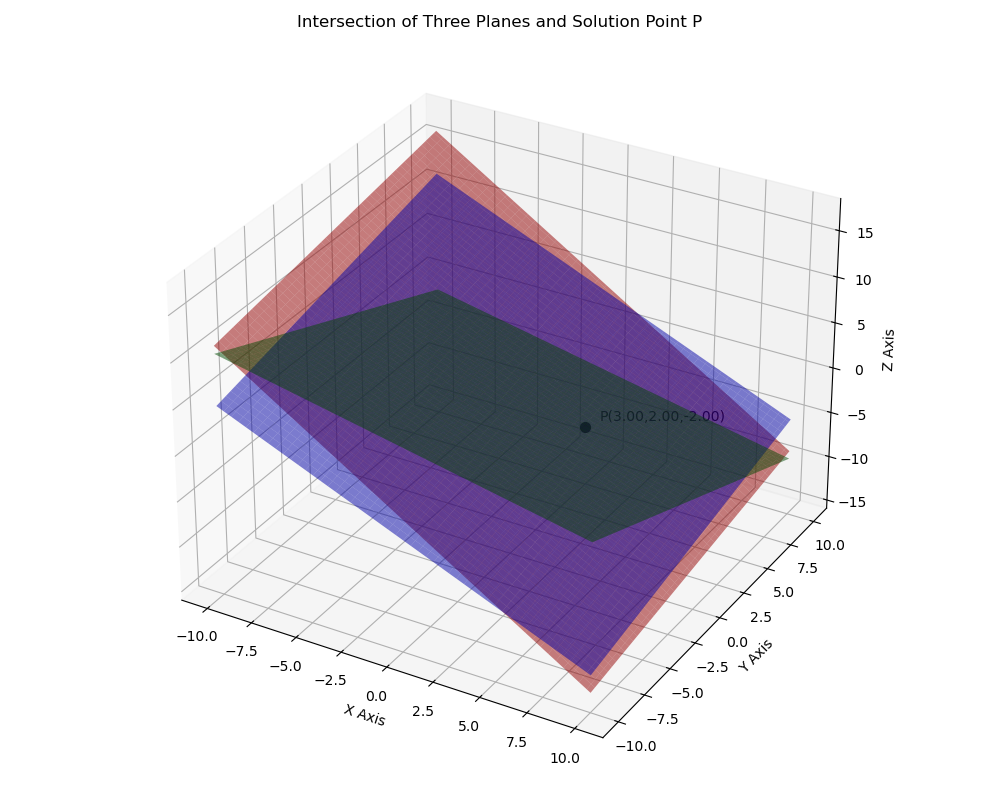
\includegraphics[width=0.8\columnwidth]{figs/Figure_1.png} 
   \caption*{Fig : Planes}
  \label{Fig1}
\end{figure}
\end{frame}

% -------------------
\begin{frame}[fragile]{C Code - points.c}
\begin{lstlisting}[language=C]
#include <stdio.h>

double *gaussian_elimination(double a[3][4]) {
    static double sol[3];
    int i, j, k;
    double ratio;
    int n = 3;

    // Forward elimination
    for (i = 0; i < n - 1; i++) {
        for (j = i + 1; j < n; j++) {
            ratio = a[j][i] / a[i][i];
            for (k = i; k < n + 1; k++) {
                a[j][k] -= ratio * a[i][k];
            }
        }
    }

    // Back substitution
    for (i = n - 1; i >= 0; i--) {
        sol[i] = a[i][3];
        for (j = i + 1; j < n; j++)
            sol[i] -= a[i][j] * sol[j];
        sol[i] /= a[i][i];
    }

    return sol;
}
\end{lstlisting}
\end{frame}

% -------------------
\begin{frame}[fragile]{Python Code - callc.py }
\begin{lstlisting}[language=Python]
import ctypes, os
import numpy as np
import matplotlib.pyplot as plt

figs_folder = os.path.join("..","figs")
os.makedirs(figs_folder, exist_ok=True)

lib = ctypes.CDLL("./points.so")
lib.gaussian_elimination.restype = ctypes.POINTER(ctypes.c_double)
lib.gaussian_elimination.argtypes = [((ctypes.c_double*4)*3)]

aug_matrix = ((ctypes.c_double*4)*3)()
aug_matrix[0][:] = [5, -1, 4, 5]
aug_matrix[1][:] = [2, 3, 5, 2]
aug_matrix[2][:] = [5, -2, 6, -1]

sol = lib.gaussian_elimination(aug_matrix)
solution = [sol[i] for i in range(3)]
x, y, z = solution
print("Solution from C:", solution)
\end{lstlisting}
\end{frame}

% -------------------
\begin{frame}[fragile]{Python Plot Code - plot.py}
\begin{lstlisting}[language=Python]
import os
import numpy as np
import matplotlib.pyplot as plt

figs_folder = os.path.join("..", "figs")
os.makedirs(figs_folder, exist_ok=True)

A = np.array([[5,-1,4],[2,3,5],[5,-2,6]], dtype=float)
b = np.array([5,2,-1], dtype=float)
solution = np.linalg.solve(A,b)
x,y,z = solution
print("Solution from NumPy:",solution)

x_vals = np.linspace(-10,10,100)
y_vals = np.linspace(-10,10,100)
X,Y = np.meshgrid(x_vals,y_vals)

Z1 = (5 - 5*X + Y)/4
Z2 = (2 - 2*X - 3*Y)/5
Z3 = (-1 - 5*X + 2*Y)/6

fig = plt.figure(figsize=(10,8))
ax = fig.add_subplot(111,projection="3d")
ax.plot_surface(X,Y,Z1,alpha=0.5,color="red")
ax.plot_surface(X,Y,Z2,alpha=0.5,color="green")
ax.plot_surface(X,Y,Z3,alpha=0.5,color="blue")
ax.scatter(x,y,z,color="black",s=50)
ax.text(x+0.5,y+0.5,z+0.5,f"P({x:.2f},{y:.2f},{z:.2f})",fontsize=10)
ax.set_xlabel("X Axis"); ax.set_ylabel("Y Axis"); ax.set_zlabel("Z Axis")
ax.set_title("Intersection of Three Planes and Solution Point P")
plt.tight_layout()
fig.savefig(os.path.join(figs_folder,"solution.png"))
plt.show()
\end{lstlisting}
\end{frame}

\end{document}
